\documentclass[10pt,twocolumn]{article}

% use the oxycomps style file
\usepackage{oxycomps}

% usage: \fixme[comments describing issue]{text to be fixed}
% define \fixme as not doing anything special
\newcommand{\fixme}[2][]{#2}
% overwrite it so it shows up as red
\renewcommand{\fixme}[2][]{\textcolor{red}{#2}}
% overwrite it again so related text shows as footnotes
%\renewcommand{\fixme}[2][]{\textcolor{red}{#2\footnote{#1}}}

% read references.bib for the bibtex data
\bibliography{references}

% include metadata in the generated pdf file
\pdfinfo{
    /Title (League of Legends Pro-Based Companion App)
    /Author (Roberto Villegas Jr.)
}

% set the title and author information
\title{League of Legends Pro-Based Companion App}
\author{Roberto Villegas Jr.}
\affiliation{Occidental College}
\email{rvillegas@oxy.edu}

\begin{document}

\maketitle

\section{League of Legends}

League of Legends is one of the most popular games in the world, with millions of active players everyday.
It is a 5v5 battle arena game in which teams fight each other to destroy the other team's base in order to claim victory.
The game, in addition to being a relatively open map for players to move in, also allows players to buy items, boosts their own stats with "runes", and capture different objectives to gain an advantage over the other team.
Because of this, you can never expect two games to end up the same way, adding to the fun of playing the game.

League of Legends also boasts one of the most popular esports scenes on the internet, with this year's (2023) world final peaking at 6.4 million viewers (not including Chinese viewership, which is certainly in the millions range)\cite{EsportsChartsWorlds2023}.
Franchised leagues are operated all around the world, from Los Angeles to Berlin to Shanghai.
Some players have even made themselves a household name, like the 4-time world champion Faker in South Korea.

\section{Problem Context}
As popular League of Legends and League of Legends esports may be, the game itself is known to be difficult to master.
There are currently 166 champions\cite{LoLWikiListOfChampions} in the game for players to choose from, each with a different set of abilities to use.
There are also over 250 items\cite{LolWikiListOfItems} available in the game, as well as thousands of possible combinations for runes\cite{LolWikiRunes}.
The game forces you to make decisions at every step of the way, beginning even before you enter the battle arena itself.
For new or casual players, these decisions can be overwhelming and can impact how well they learn and play the game.
It even has an impact on how a player enjoys a game (who would enjoy a game they consistently struggle at?).

All of this combined make for a rather negative gaming experience if you are not a player that has been playing for multiple years or a player with friends to show you how to play.
And assuming that the average player will only play a few hours for a couple days a week, there are little to no ways for a player to actually improve gameplay and game experience outside of constantly playing the game and learning decision-making strategy from other players in game.
So what can a player do to improve their decision making and thus improve gameplay and game enjoyment?

\section{Proposed Solution}
My app aims to solve this problem by collecting public game data from games played by LoL esports pro players and providing suggestions to users based on this data.
It will suggest rune combinations and possible item purchases to the user based on the champion they choose and the champions they are playing against.
Pro player data will be constantly updated with the latest game data, ensuring that users will have the most up-to-date builds to choose from.

\section{Technical Overview}
There are three main things being used for this app: the Riot Games API, a MySQL database, and the League Client API.

The Riot Games API is where all of the game data will come from.
As long as I have a list of known pro player accounts, the app will be able to access data for any match a player may have participated in.
For this project, the most important data to collect from this API is which runes they have used, which items they have bought, what champions they have played against, and the end-game stats (total damage, total gold earned, etc.).'

This data will be stored in a MySQL database divided into different tables based on data type. The "Teams", "Players", and "Accounts" tables contain general data about the players and the accounts they own. 
The "Teams" table is specifically used in case a user wants to use runes from players that are part of a specific team or region.
The next set of tables are the main tables used for the app. These tables are "Matches", "MatchPicks", "MatchRunes", and "MatchItems".
The "Matches" table contains the general data of the match, including the match ID and the match timeline (more on what this is used for later).
This table is also used as a reference for the other "match" tables as a foreign key to use as a primary key.
The "MatchPicks" table stores data on what champions are picked in each match in the "Matches" table.
This also includes non-pro picks, since some suggestions will be made based on what champions pro players are playing against.
"MatchRunes" and "MatchItems" contain a list of runes and items used by the pro player in a match.
"MatchItems" also contains the order in which an item is purchased, since this is important for how a build works in LoL.

To get the data from the database to the game client itself, the app makes use of the League Client API.
This is a locally hosted API by the game client with endpoints accessible by a WebSocket.
The two-way connection provided by the WebSocket allows the app to maintain a constant connection to the client and listen for any updates, mainly updates for when a player connects to a game.
It also allows the app to create objects in the client, which will be used for adding runes pages and item sets with the suggestions.

\section{Existing Apps}
There are a few existing apps that work quite similarly to this one.
For starters, they all collect data using the Riot Games API to collect game data.
Most apps, for example mobalytics.gg and porofessor.gg, will offer different build based on what is being played the most (similar to this app).
They can take a look at what is going on in champ select and make suggestions based on what may be the best decision to make.
Even during the game, stats can be tracked to give the user an idea of where they should be in comparison to players of a similar rank.

Other apps, like op.gg and u.gg, even provide opportunities to track the pros, similar to how this app has a pro focus.
Users can use their apps or visit their website to see a list of pros that are currently playing to spectate their games, or to take a look at their match history and see what they've been up to in terms of builds and champion picks.

The key difference between these apps and my app is the fact that this app is specifically focused on collecting pro player data and making suggestions based on that.
The other apps will collect data from the entire player base and make suggestions based on what other players are finding success with.

Issues can arise from this because not every player's data can be considered reliable.
One type of player that is common to find in League of Legends is one that plays the same champion all the time, usually called a One Trick Pony (OTP).
OTPs can be notorious because these players will know every detail about the champion they play, even beyond the descriptions the game may provide.
These players will also have a unique set of builds that they may use to suit their own unique playstyle.
All of this data will be included in the general player data that these apps use for suggestions, which would give a false representation of what actually is a good build.


\section{Foundational Assumption}
An important aspect of this app to note is that there is a foundational assumption that everything relies on to justify the idea behind this app.
This assumption is that pro players make the best decisions in the game out of anyone else in the player base.

The logic behind this assumption considers the time and dedication pro players have to playing the game.
Players that go pro in League of Legends are typically the only players that will spend most of their day playing and thinking about the game\cite{KSLNewsFPX}.
It's their job; they are pretty much required to keep up with the latest trends in the game if they want to stay on top of.
Whenever they are not with the rest of their team for team meetings, practices, or scrimmages with other pro teams, these players spend their time playing in the solo competitive game queue to refine their gameplay.
Because of this, I believe it is safe to assume that anything they do when playing the solo game mode can be considered the "correct" decision to make in whatever situation they're in.
This includes runes selected and items purchased.

This assumption has its fair share of flaws, though.
A question I was asked in regards to this assumption considered how much of an effect a pro player's own mechanics have on the success of a certain build.
In other words, how do we know a certain build is actually a good build and not just a result of the player's high skill level?
Will the pro player's success with a build translate to a user's success when they use the same build?
This is similar to the issue I raised regarding OTPs for other similar apps.
It is difficult to confidently answer this question because there is no reasonable way for me to determine where the success of the build is coming from.
I don't have access to a pro player's mouse and keyboard input to compare their game mechanics to a user's mechanics.
I'm not in the room when a pro player is playing the game, so the "why?" behind all of their decisions is lost.
It's not possible for me to differentiate between a good build and a good player, so this question will unfortunately remain without a complete answer.

However, I still believe it's reasonable to prefer using builds from pro players rather than the general player base.
Another trait of pro players is their reliability to understand multiple different champions in the game and play them proficiently (by pro standards at least).
Sometimes, a pro player will be asked by their coach to play a certain champion because it fits in well with the rest of the team's composition, even if the pro player may not be the "best" or at least comfortable with that champion.
Even in this situation, the pro player will know how to play the champion and what to build because of their expertise in the game.
So, when a user needs a build and is given something a pro player used, they can safely assume that it is an acceptable build.
A build from any other source may not be as reliable.


\section{Methods}
My approach to the app focuses on layering the different functions of the app on top of each other based on importance.
At the very top is the connection to the League Game Client.
All input to the app originates from the client, so connection to the client will remain at the highest level of the app.
Everything goes through the client control.

Next is the part of the app that controls what happens during the champ select phase of the game.
Before every game, players have a chance to choose their champion to play, as well as edit their runes page to adjust their champion stats and passive abilities.
This is the main part of the app where suggestions are produced and given to the user.
Input from the client is passed through this champ select control section, passed to the database for relevant data, and uses the resulting data to pass a suggestion back to the client for direct implementation.

Last is the database control section of the app.
This is the only part of the app that has direct access to the database in order to regulate the data that comes out of the database, as well as make it easier to send queries with different parameters and requirements.
Whenever the champ select control section needs data, a function from the database control is called, which sends the query with the correct parameters and returns the result.
The result that it sends can change depending on what is needed in the champ select control section(more on this below).

\subsection{League of Legends Game Client}
The entire app relies on its connection to the game client.
As such, establishing a WebSocket connection between the app and the game client is the first step when starting the app.

When the app and the game client are both running, the app establishes a WebSocket connection and a "GET" request is made for the current user's account information.
Some request require information like the user's "summoner ID" ("summoner" is the game's way to call players) when requesting information, even though there is only one account logged in to the client at any time.

After this is done, another connection is established with the champ select endpoint in the client.
This is the only endpoint that has a constant connection since any phase of champ select will indicate when a lobby has been joined or a game has started.
When an update is sent to this endpoint, the update is read to check what exactly is going on within the client.
If the champ select phase has started, a call to the champ select control section is made and the suggestion process starts. 

\subsection{Champ Select}
Depending on which phase champ select is currently at, a different function may be called.
For example, if champ select just started and there are not any picks yet from either team, the all the app can do is suggest a champion to pick based on nothing but popularity and success.
When an enemy pick is finally made, then more specific suggestions can be made to possibly counter what the enemy team has already picked.
This will continue until the user makes a pick of their own, which will shift the focus of suggestions from champions to runes.

The app will still have to consider what the other team has already picked, since runes can change depending on who a player is playing against.
Three different suggestions will be made: the most popular runes build for that champion (regardless of success or enemy picks), the most successful in terms of individual performance (regardless of enemy picks), and the most successful versus the likeliest lane opponent.
It is impossible to know for sure which champion in the other team will be your lane opponent because the client hides the position of the other team.
Certain champs can even be played in different positions, so the app will have to take a look at the enemy team and decide who might be the user's lane opponent.

Once all picks have been made for both teams, final suggestions will be sent to the client for the user to choose from before the game starts.
The user will have full control of what build they want to use in case they have a specific playstyle they want to use for that game.
If the player does not have the game knowledge to know what they want or don't want, there is always the "most popular" build for them to choose from.

\subsection{Database}
In order for the champ select control section to make suggestions, it needs access to the data in the database.
This database control section takes input from the champ select control section and makes queries to the database based on which function is called and what parameters are added to the call.

The database is organized in a way to make the results of queries easier to process by the champ select control section.
To start, the runes chosen by a pro player in a game are stored in one row.
This is because runes are typically done in groups (primary runes set, secondary runes set, and "stat" runes set) so storing runes individually would not produce correct results.
When stored in one entry like this, an accurate representation of the most popular/successful runes can be generated and sent to the champ select control page.

Items on the other hand are stored as individual entries in the items table.
This is because items can be bought without consideration for any other items that are purchased.
When a list of items needs to be generated, one query can be sent to find out which item is the most purchased item for a champ in a specific position.
Then, another query can be made to see the next most popular item purchased, but this time it must be an item bought with the first item.
Rows for items are stored with match and player information, so it is no issue figuring out which items are bought with which items.

Lastly, the table of champion picks themselves are stored in their own table.
This contains not only pro player picks but also non-pro ally and enemy picks.
This is because it is important to know who a pro player has played against when they decided to use a certain item or rune build.
This is also what is used for builds specific to success versus another champion.

A few different ways of organizing the database were considered when figuring out what would be most efficient.
In the initial design, an entire build for a champion was included in one row per pick.
This included the champion picked, the runes they used, and even the items they bought that game.
This was a problem though, because there was no way to tell who that player played against.

When champion picks were separated from the rest of the build, another issue was encountered with the items.
Originally, only 6 columns were reserved to store what items a player purchased in a game.
This on its own wasn't too much of an issue until I realized there had to be something that separated items by type.
In the game, there are different types of items that can be built at different points in the game.
"Starter" items, for example, are available for a player to buy at the beginning of the game to have basic stats and abilities enhanced until they can buy real items later in the game.
"Mythic" and "Legendary" items are the highest tier of items you could get, which all have special effects in addition to the stats and abilities they provide. 
Between "starter" and "mythic"/"legendary" items are "basic" and "epic" items, which are used as components to build the higher tier items. 
Multiple high tier items can use the same "basic" and "epic" items as components, which caused problems for generating item lists when they were in the same row.
At first, popular item builds were missing because having a lower tier item would make the app not recognize the build as the intended build.
These lower tier items would also make their way to the items list sent for suggestions, which didn't make sense because there is no indication as to what item it should be built into.
As a result, I separated items into their own table with each item having their own row.
In this way, the item tier can be stored as its own column, making queries easier and more direct.
The item build order is also possible since this can be another column as well.
The result of these changes are three different tables for picks, runes, and items for easy query. 

This database control section will always have access to the database during the entire champ select phase, so any and every update made in the champ select control section of the app will be able to request new data for new suggestions until it is time to start the game.

\section{Evaluation}
To evaluate the effectiveness of the app, an analysis of the user's build in a given match will be required.

\subsection{Ineffective Evaluation}
It will be difficult to define effective evaluation metrics for this app based on user performance because there are so many factors that can go in to how well a player does in a match.
Especially since LoL is a team game, there are some situations you simply cannot avoid because of a teammate's poor performance and decisions.
It is possible to win with a poor individual performance, and it is possible to lose with an extraordinary individual performance.
As such, a player's winrate will not be used to measure the app's success.

Additionally, using a player's stats at the end of the game (total damage dealt, kill/death/assist ratio, etc.) is also not the best way to determine build success.
Similar to the issue with using a player's winrate, there are too many factors that can affect player stats.
In a losing game, you are more likely to have more deaths than when you win.
You are also more likely to have poor damage stats, since the enemy team likely was much stronger than you by the end of the game.
While endgame stats may be more reliable than a winrate analysis, I still think there can be a better way in assessing a build's success.

\subsection{Evaluation Metrics}
With the previously mentioned concerns in mind, I have come up with metrics that are difficult to be affected by outside factors.
Instead of focusing on the user's stats, my evaluation of the project will focus on the effectiveness of the items and runes against enemies.

To elaborate, the evaluation process will take into account the state of each participant in a game and calculate the damage of the player's abilities and attacks against each enemy.
The "state" of a participant simply means checking the runes and items a player has, the champion they are playing, the champion's level at a given point in the game, and more.
But why is this a better evaluation metric compared to the ones before?
The general idea is that certain builds are used because they are considered the best in a given situation.

To illustrate, I want to focus on one item in the game called "Lord Dominik's Regards" (LDR for short).
The most important stat and effect the item gives players is 35\% armor penetration and 0-15\% bonus damage against enemies with greater maximum health.
So if an enemy has 300 armor and 1000 more maximum health than the user, their armor is effectively reduced to 195 armor and the user gains 7.5\% bonus damage against that enemy\cite{LolWikiArmorPenetrationCalculation}.
The item also gives the user 40 attack damage and 20\% critical strike chance, which means this item is most effectively used by the "attack damage carry" role player in a game.
This item is obviously most effective when used against high health, tank enemies in a game, especially late in the match.
It is not very effective outside of this, which can be a waste of money and time for the user if they don't build it in the right situation.
For example, if the enemy only has 50 armor and does not have greater maximum health, then their armor is only reduced to 32.5 and there is no bonus damage.
The value and effectiveness of the item against an enemy is greatly reduced.

So, when you combine and calculate the damage of all items and runes a player has at a certain point in the game against an enemy, you can see how effective the build is.
Even if a game is not going well and the user may not win or have the best final stats in the game, the damage of a build will tell if it is effective or not and imply whether or not the build was good to go with.

\subsection{Evaluation Method}
Using the evaluation metric explained above, we will need a player's champion, a list of enemy champions, and the state of that player in multiple points of the game.
I made a script to help with this process, which creates a Match object containing general match data, and a list of Participant objects for everyone in the game.
Each participant has a timeline that contains their state in one minute intervals from the beginning of the game to the end.
Using a custom damage calculator script, each minute of the game will be analyzed to see how much damage the user's attacks and abilities can do to an opponent.
It doesn't matter which champion the user is playing as or against since build effectiveness is not exclusive to individual champions.

Using these calculations, you can look at a user's games before using the app and compare it to games with the app to see how much of a difference in damage there is.

\subsection{Final Evaluation}
A successful evaluation of the app would mean seeing some kind of improvement in the damage a player can do as compared to without the app.
The actual amount of improvement can vary; for losses, the improvement can be a rather small change.
In wins, the improvement can be a very large and clear as compared to before.
As long as there is a general increase in damage per ability, I would consider that a success.

If the amount of improvement stays to be a small amount across all situations, or in a worst case scenario, damage actually worsens, then we can say the app is not accomplishing what I was aiming for.
With all the factors that may affect a build's effectiveness, a situation with little or no improvement would point at the build not being good, since that is the only common factor in those games.

For this app specifically, I will be using my own game data comparing stats before using the app for builds and while using the app.

\section{Results}
We will be looking at three different pairs of games played with the same champion.
One game is without the help of the app, and the other is with the app.

\begin{figure}
    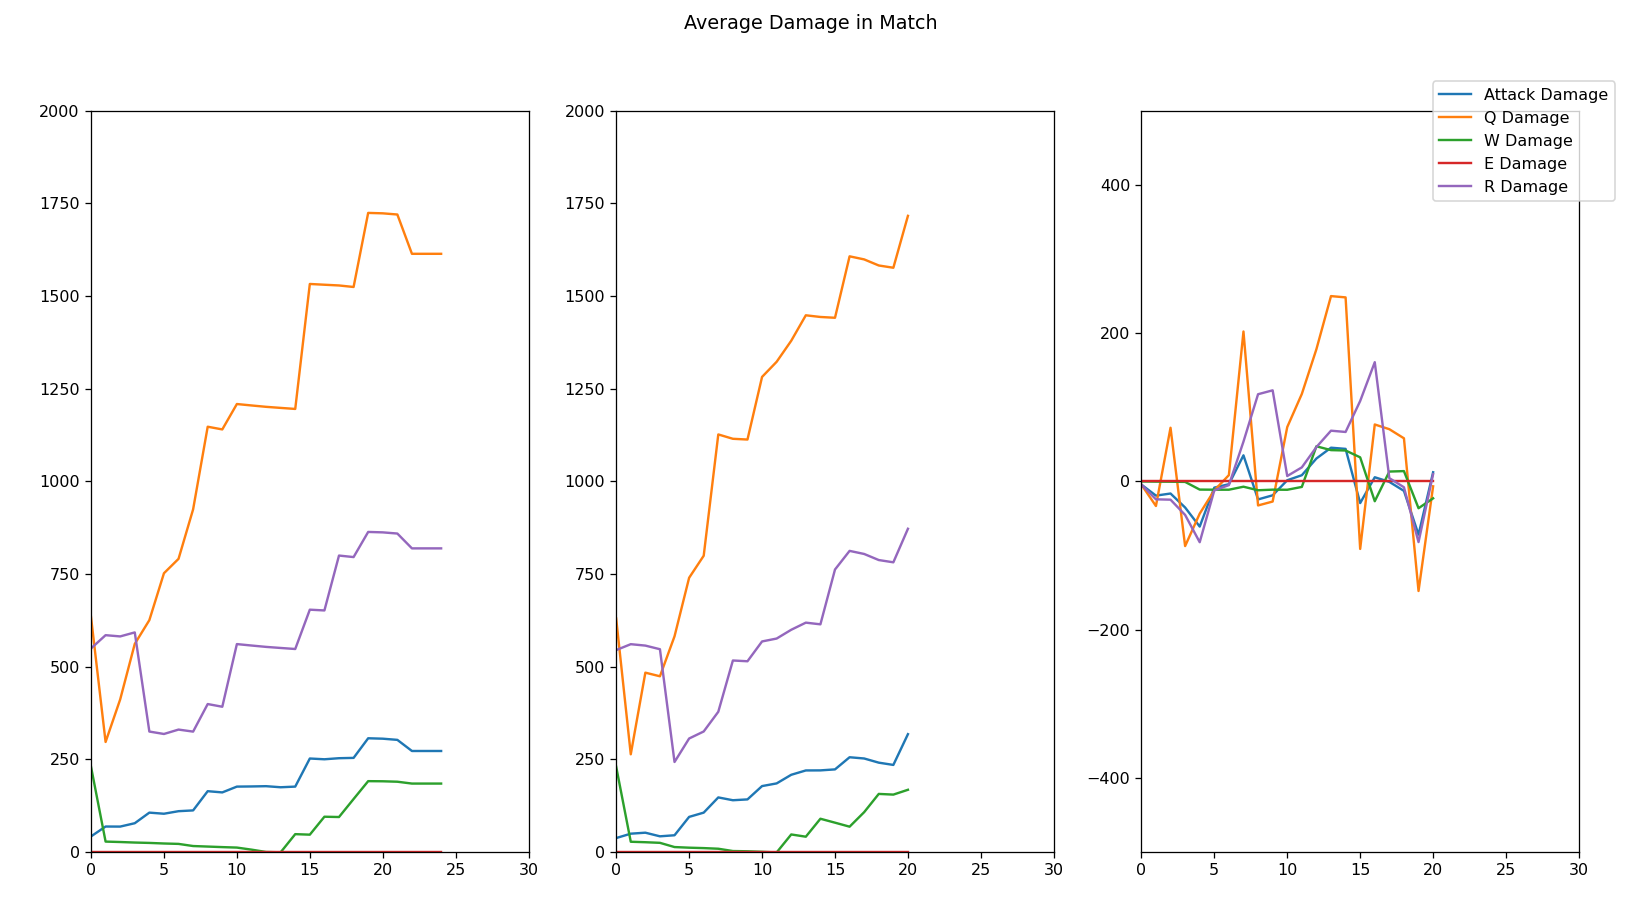
\includegraphics[width=.95\linewidth]{GravesDamage.PNG}
    \caption{Graves Damage Comparison}
\end{figure}

\begin{figure}
    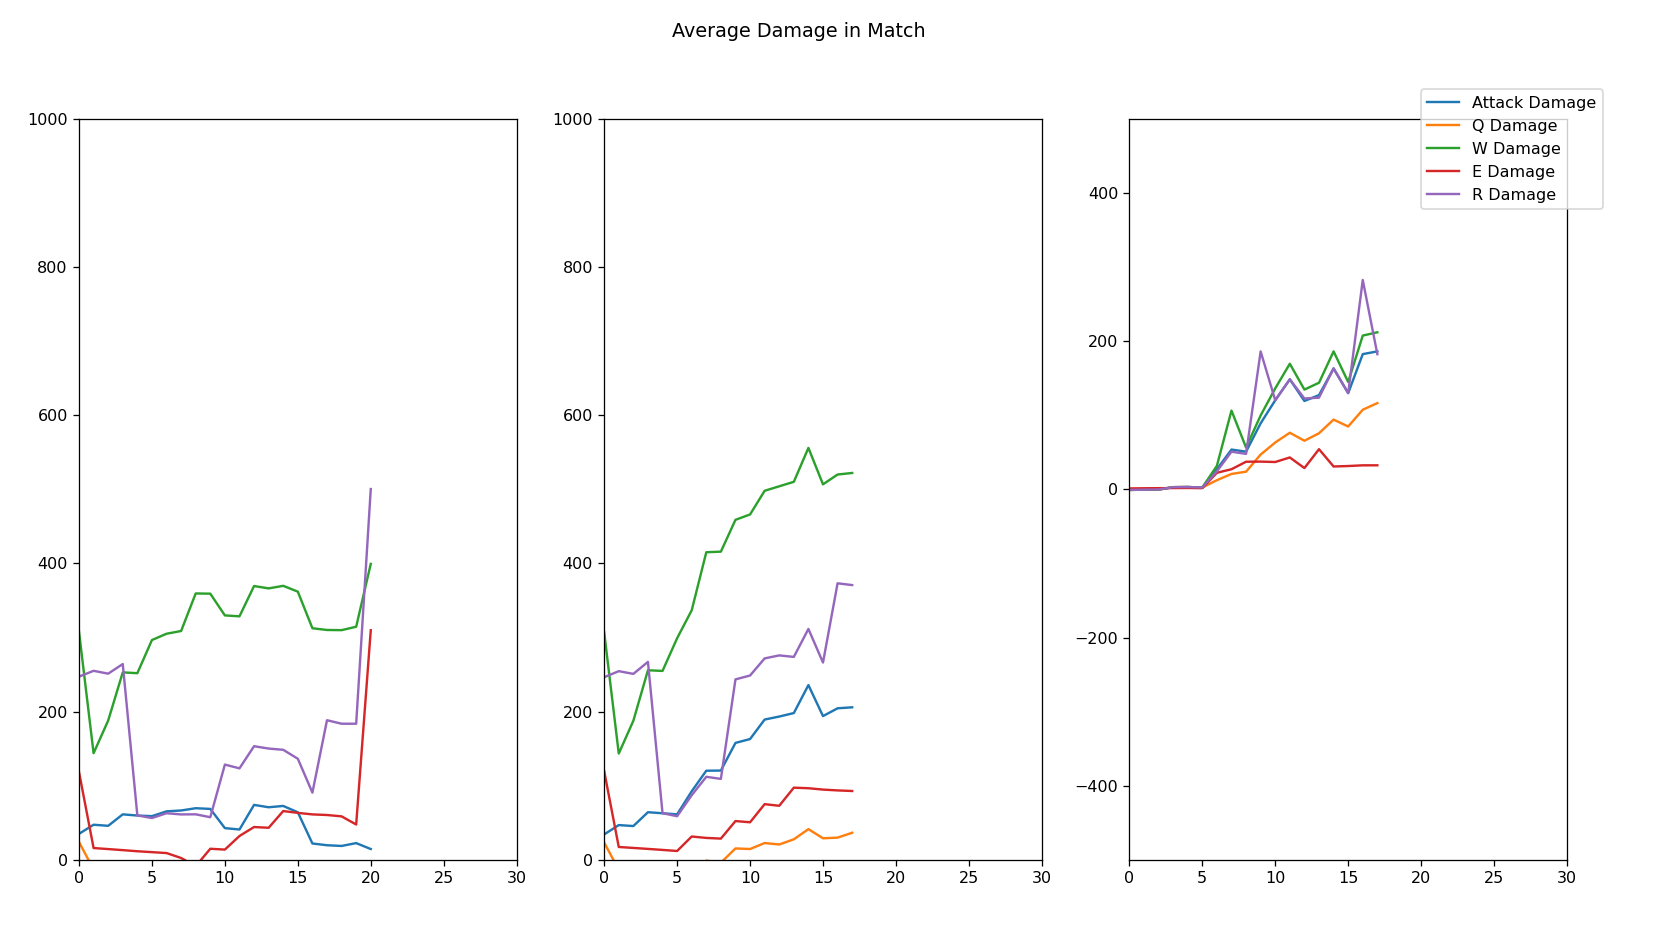
\includegraphics[width=.95\linewidth]{XinZhaoDamage.PNG}
    \caption{Xin Zhao Damage Comparison}
\end{figure}

\begin{figure}
    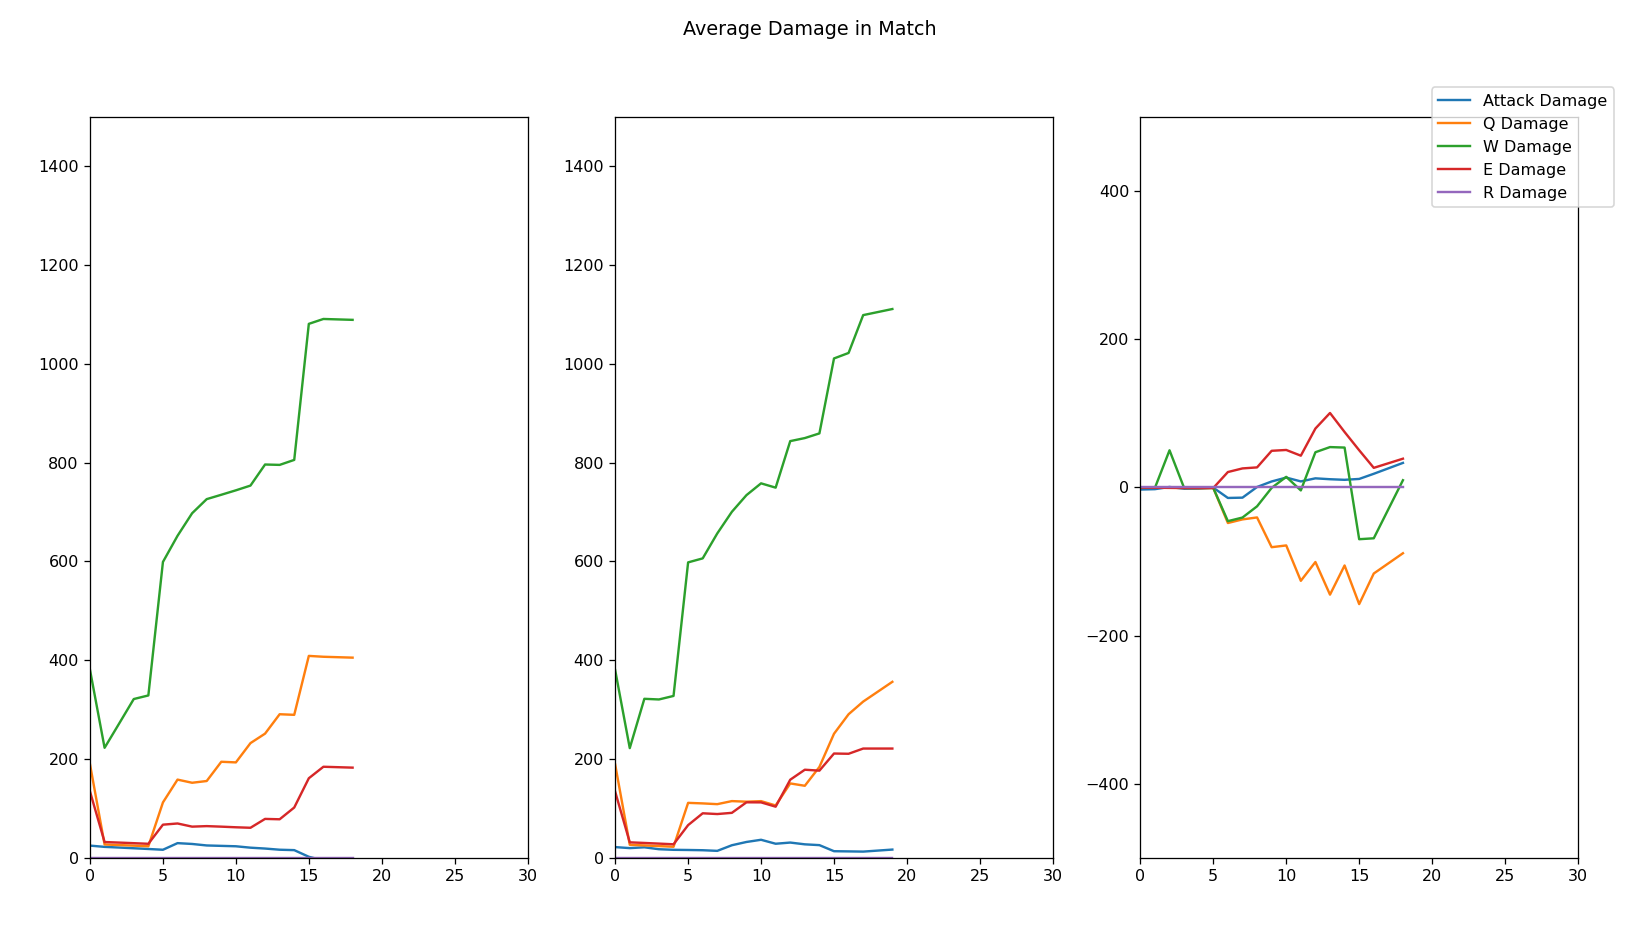
\includegraphics[width=.95\linewidth]{TwistedFateDamage.PNG}
    \caption{Twisted Fate Damage Comparison}
\end{figure}

\subsection{Analysis of Results}
Each figure has three charts: one with average damage from the match without the app, one with average damage from the match with the app, and a third chart showing the difference between the first and second charts.
"Average Damage" simply means the average damage an attack and each ability can do to enemy champions.
So if an attack does 10 damage to one enemy, 20 damage to two other enemies, and 30 damage to the last two enemies, the average damage would be 22.

Starting with the first one (the "Graves" chart), we can notice that both charts seem to have generally similar trends.
This applies to all three examples, and it is simply because the base damage of each ability scales the same throughout the game and will give similar trends for each match.
We can also notice in the Graves example that, while there are fluctuations between positive and negative damage difference, there are higher peaks in the positive side.
What this means is that purchasing an item according to the recommended build by the app will yield a higher efficiency item, since you are spending the same money for more damage.
This is generally what I am looking for in the evaluation of the app.
A higher damage output means getting kills easier and faster, more money, and more items, allowing a user to snowball their game to a win.
A quick note about the "E" ability remaining at 0: abilities that don't do any damage are still included in the chart and will remain as an y=0 line in every chart.
This chart's data can be found as json files titled "NA1\_4948110139.json" and "NA1\_4948918567.json".

Moving on to the Xin Zhao chart, this analysis is pretty straight forward.
Every ability yields more damage in the app-assisted game as compared to the non-app game.
The gains aren't as significant as I would maybe hope for them to be (all hovering at or below 200 damage), it is still all positive and could be considered successful.
Overall, this worked mostly as intended.
This chart's data can be found as json files titled "NA1\_4948094107.json" and "NA1\_4948906044.json".

And the last chart, the Twisted Fate chart, is a little bit more even than the previous two.
The most prominent detail about this chart is the negative "Q Damage" line, meaning that the non-app match had higher "Q" damage than the app-assisted match.
Even if both builds focus around higher attack damage, which is supported by the positive "Attack" and "E" (an attack-based ability) damage lines, the dramatic drop in "Q" damage is concerning.
Could the build be bad?
Maybe that specific game was not the best situation for the build?
In any case, it's reason enough believe that the app could use some improvement, whether its a better recommendation system or more data to calculate from.
This chart's data can be found as json files titled "NA1\_4946973385.json" and "NA1\_4950877410.json".

\subsection{Conclusion}
Overall, I believe this showing of the app is not a bad start.
Generally, it is giving decent recommendations that have the potential to improve a user's damage output and thus gameplay.
There is a lot that could be improved though, including better enemy analysis to recommend more influential items and runes.


\section{Ethical Consideration}
It is difficult to accurately recognize the possible biases and contributions to inequality that the app may have because of the fact that it is a companion app to a video game.
Thus, to start, any ethical issue tied to League of Legends will be tied to the app even if it does not have a direct connection to that issue.

The first possible consideration for the app could be its physical accessibility.
Can users with physical disabilities use the app to its full capabilities?
In short, yes.
But it is contingent on if the user is able to play League of Legends in the first place.
The game does not use the same general controls(buttons to move in four directions, buttons for different actions, etc.) that most games use.
For example, movement in League of Legends is based on where you right click in the map.
Wherever you click, you move to that position.
But you can also left click an object or enemy to start attacking them.
Your cursor position is also used to aim abilities, which are casted by pressing keys.
Even moving the in-game camera is controlled by your mouse movement unless you have the locked camera setting enabled.
With all these issues, if a user has found a solution to play the game without any obstacles, then the app will work for them as normal.
Fortunately, the app works by inserting the data directly into the game client itself, so any external windows or programs are not necessary.
As long as a user has adequate access to the game, then they have adequate access to the app.

There is significant consideration to be had with the competitive advantage the app may provide, though.
Riot Games provides quite little guidelines on what is allowed for third party applications that can affect gameplay, but it is relatively straightforward \cite{RiotGamesThirdPartyApplication}.
Their websites states that an app can't provide a "measurable player advantage."
This includes:
\begin{itemize}
    \item Exposing information that’s intentionally obfuscated (cooldowns or timers)
    \item Taking actions on your behalf (botting or scripting)
    \item Drawing conclusions for you (predicting enemy positions)
    \item Altering your field of intelligence (zoomhacks or global ult alerts)
\end{itemize}

None of these are an issue with this app.
All the app simply does is provide information to the user for them to make decisions.
The user can even decide to not use the provided suggestions if they didn't feel like using them.
There is no information provided by the app that is hidden by the game client, so any unfair advantage is avoided by the app.

\section{Appendices}

\subsection{Replication}
First, the correct version of Python needs to be installed.
The version used for this project was 3.10.5.

A MySQL instance is the next item needed to be installed for the app.
The version of MySQL used to make this app is version 8.0.34.

Lastly, the dependencies used by the app are listed in the requirements.txt file.
There are two areas where this can be done, one in the "app" folder and one in the "evaluation" folder.
When developing the project, I used two different virtual environments for each folder.
Anyone wishing to replicate the app can run "pip install -r requirements.txt" which will pip install everything needed to run the app.

After everything has installed, it is time to fill the database.
In the app/database folder, a SQL file is provided, which takes care of creating the database with the necessary tables.
You can do this using the MySQL instance installed previously.
After the database is up, the first script to run is update\_accounts.
This will fill the Accounts table with the necessary data for the rest of the tables to be filled.

Before running the following scripts, you must first secure a RiotAPI key and place a "RiotAPIKey.txt" file containing the key in the "evaluation" and "app/database" folders.
This will allow you to access the API that will provide all of the match data used in the app and evaluation.

The next (and last) script to be run is the update\_matches script.
This will fill the Matches, MatchPicks, MatchRunes, MatchItems, and MatchStats tables.
These are the main tables used to send data through the app and to the game client.

Once everything has been set up for the app, you can start the app by running the lcu\_control script.
Of course, to actually make use of the app, you will need to have League of Legends installed on your machine.

\subsection{Code Architecture}
The first component of the app's code is the lcu\_control python script.
After connecting to the client, the only endpoint that it connects to is the champ select endpoint.
Still, there are still a few "get" requests that the script makes to collect data, based on the phase of champ select that the game is currently in.
For example, when there is any update to champ select, the script will make a "get" request to that champ select endpoint in order to get the phase of champ select.
When this has been secured, the phase of champ select is checked and additional "get" requests are made.

This script is the only one that has access to the client because it keeps the code organized without every script in the project having access to the client.
It avoids having possibly redundant code and keeps the source of champ select data in one place.
No unnecessary calls are made to the client.

The db\_control script is the only one with access to the database for the same reason.
There are no unnecessary connections to the database for extra queries.

The script connecting client data to database data is the champ\_select\_control script.
It takes in client data based on the function called by lcu\_control, and makes the relevant request to the database by calling a function from db\_control.


\printbibliography

\end{document}
